\title{Decentralised location proof system}

\documentclass[12pt]{article}

\usepackage{tikz}
\usetikzlibrary{calc,arrows}
\usepackage{enumitem}
\usepackage{float}
\usepackage{enumitem}

\setlist{parsep=0pt,listparindent=\parindent}

\begin{document}
\maketitle

\begin{abstract}
\end{abstract}

\section{Introduction}

\section{Previous work}
Location proof systems are expected to be accurate and tamper-proof. For this reason, existing solutions have chosen to use a central authority to issue proofs \cite{brassil, luo, khan}.

Hardware techniques \cite{brassil} operate by supplementing existing WiFi access points with \textit{femtocells} (small cellular antennae that connect to the mobile carrier via the Internet). Location verification over the internet is made possible by determining which femtocell a mobile node is connected to as it transfers data via Wi-Fi. This solution requires investment in additional hardware to supplement existing WiFi access points. It also requires access to mobile providers user database to identify users locations.

Other proof systems \cite{luo} deploy software on Wi-Fi access points. Access points taking part in the location proof network become part of a 'group' with a shared group signature. Mobile nodes can request a location proof from an access point, who signs it with the group signature. Access points provide location proofs to nodes without ever learning the node's identity, thus protecting user's privacy. However, due to the system’s reliance on the group signature structure, access points become a target for attack. Compromising an access point would allow an attacker to create false location proofs.

\cite{luo} considers a number of threats in their architecture:
\begin{itemize}
	\item \textbf{Dishonest users.} A dishonest user tries to obtain location proofs that certify her presence at some place at a particular time even if she was not there. Dishonest users may achieve this goal by colluding with malicious intruders.
	\item \textbf{Malicious intruders.} A malicious intruder is not interested in obtaining location proofs for her own use but offers to help other users to get location proofs on their behalf in exchange for other benefits like money.
	\item \textbf{Curious APs and applications.} A curious AP tries to learn a user’s identity while the user is acquiring a location proof from the AP. Similarly, a curious application tries to learn more location information from a location proof than it really needs.
	\item \textbf{Malicious applications.} A malicious application obtains location proofs from its users and then tries to take advantage of these proofs to get unauthorised access to other applications.
	\item \textbf{Active and passive eavesdroppers.} An eavesdropper records and maybe modifies communication between users, proof- ssuers, or applications.
\end{itemize}

Distributed P2P location proof systems also exist \cite{khan}. A central authority is used and acts as a certificate authority, issuing a unique ID to each person using the system. Unique identity is proved by users by providing SSN, driver’s licence, or passport documents. This removes the threat of a Sybil attack \cite{sybil}, but makes the central authority a clear target for attack. The system uses three parties to provide location proofs; a mobile user who requests a proof, a fixed location authority, and a mobile user who acts as a witness. The system becomes vulnerable in the case where all three users collude, but is otherwise quite an interesting approach.

\cite{khan} also outlines a number of possible attacks on their system:
\begin{itemize}
	\item \textbf{False presence:} A malicious user can create a fake location proof on his own, without being physically present at the location. The fake proof is supposed to resemble an actual proof, which the user could have actually collected from a valid location authority.
	\item \textbf{False timestamping (backdating, future dating):} In a backdating attack, the user and the location authority colludes to create a proof for a past time. Conversely, in future dating, the location authority and a user colludes to generate a proof with a future timestamp.
	\item \textbf{Implication:} A location authority and/or a witnesses can falsely accuse a user of his presence at a certain location. In this case, the malicious location authority and witness colludes to generate a false proof of presence for the user.
	\item \textbf{False assertion:} A user can collude with a witness, and generate a falsely asserted location proof. The truth value in such a fake proof is reinstated with the assertion received from the other user.
	\item \textbf{Denial of presence:} A user can visit a location and at a later time, deny his presence at that location. In such a case, the user actually denies the validity of a certain location proof that has been been generated upon his presence at that particular location.
	\item \textbf{Proof switching:} The user is expected to have full access to all storage facilities on his mobile device. Hence, the user utilizes the legitimate proof and manipulates the information to create a false proof for a different location.
	\item \textbf{Relay attack:} A user can use a proxy to relay the requests and collect a location proof. Alternatively, a location authority can maliciously relay assertion requests with the witness not being present at the site.
	\item \textbf{Sybil attack:} A Sybil attack occurs when a single user generates multiple presence and identities [29]. A user can launch a Sybil attack by generating multiple identities representing a user and a witness and provide false endorsements for location proofs.
	\item \textbf{Denial of witness’s presence:} At the time of proof verification, the user can claim the absence of witnesses at the site or falsely claim an assertion to be counterfeit. The user and the location authority may also collude and claim the non-availability of witnesses.
	\item \textbf{Privacy violation:} An attacker may capture an asserted location proof generated for a user, and discover the identity of the user and/or the witness.
\end{itemize}

'OTIT' \cite{otit}, a model for designing secure location provenance, can be used to compare existing location proof systems. This model defines the following requirements necessary for designing any secure location provenance scheme: Chronological, Order Preserving, Vereifiable, Tamper Evident, Privacy Preserved, Selective In-Sequence Privacy, Privacy Protected Chronology, and Convenience \& Derivability.

\newpage
\section{Design}
The location proof system we propose allows mobile nodes to create location proofs for each other after physically meeting. When two nodes are in close physical proximity, they initiate a transaction over a short range, ad-hoc network such as bluetooth.

To create a transaction, two nodes anonymously agree upon their location and current time over a short-range network. Once both nodes agree upon these parameters, they each create an encrypted, privacy-protecting transaction logging their location and the alibi used to create the transaction. This transaction is published onto a public, append-only bulletin board known as a \textit{blockchain}. Once given permission and decryption keys from a node, a \textit{verifier} can determine whether or not the node is present at its claimed location.

Any node acting as an alibi in a transaction will share details of its most recent transactions with the other node in the transaction. This allows the verifier to be given permission to check the authenticity of all recent alibi's, and each of the alibi's recent alibi's, etc. Only the owner of the transaction can give permission to a verifier to check its location history, by providing the verifier with the keys needed to decrypt the transactions.

\subsection{Identities}
In order to preserve user's privacy, a user will only ever use an identity for one transaction, before generating a new one. This prevents malicious users from watching the public blockchain for a known identity and tracking it. However, to prevent identity theft, it is important for the verifier to be able to prove that a node was the original creator of each identity. This is achieved using a public/private key pair for each node.

% add nonces and PK verification to the verify_request diagram! and discuss them below!

When a node is created, it generates a key pair. To maintain anonymoty, the node will use the public key to encrypt some nonces to create identities, and use these identify itself in a transaction. During the verification stage, the node will provide the verifier with its public key, along with the list of the nonces used to generate its $n$ most recent transactions. The verifier calculates the node's identities using the public key and nonces, and retrieves the relevant transactions from the public blockchain. The verifier will also ensure that the node owns the private key associated with the provided public key, to prevent identity theft.

\subsection{Transactions} \label{sec:transactions}
During a transaction between two nodes, a number of different items must be shared and calculated. Figure \ref{fig:transaction} describes an honest, successful transaction, assuming an ad-hoc bluetooth network has already been set up between nodes $A$ and $B$.

\begin{figure}[h]
\resizebox {\columnwidth} {!} {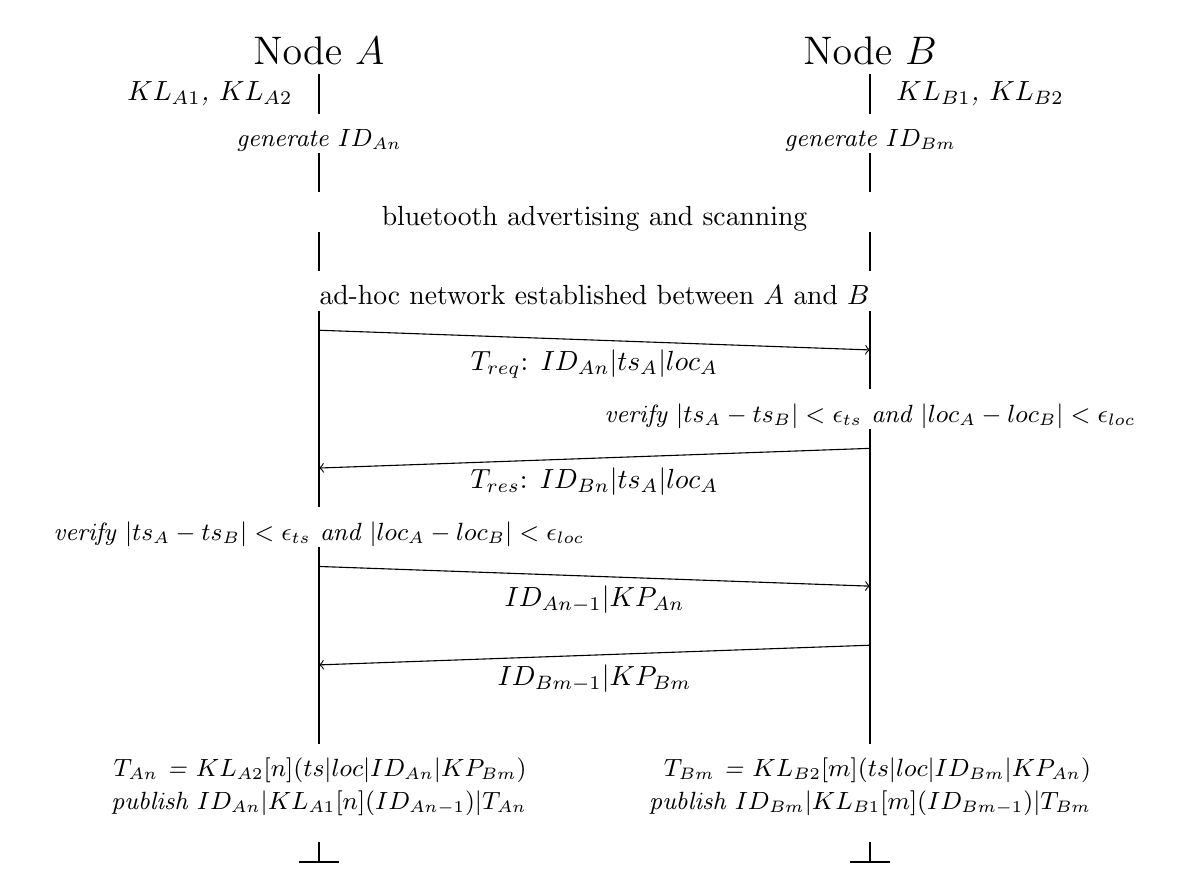
\begin{tikzpicture}
\coordinate (A_1) at (0,10);
\coordinate (A_2) at (0,9.5);
\coordinate (A_3) at (0,9);
\coordinate (A_4) at (0,8.5);
\coordinate (A_5) at (0,8);
\coordinate (A_6) at (0,7.5);
\coordinate (A_7) at (0,7);
\coordinate (A_8) at (0,4.5);
\coordinate (A_9) at (0,4);
\coordinate (A_10) at (0,1.5);
\coordinate (A_11) at (0,0.25);
\coordinate (A_12) at (0,0);
\coordinate (AF_L) at (-0.25,0);
\coordinate (AF_R) at (0.25,0);

\coordinate (M_1) at (3.5,8.5);
\coordinate (M_2) at (3.5,7.5);

\coordinate (B_1) at (7,10);
\coordinate (B_2) at (7,9.5);
\coordinate (B_3) at (7,9);
\coordinate (B_4) at (7,8.5);
\coordinate (B_5) at (7,8);
\coordinate (B_6) at (7,7.5);
\coordinate (B_7) at (7,7);
\coordinate (B_8) at (7,6);
\coordinate (B_9) at (7,5.5);
\coordinate (B_10) at (7,1.5);
\coordinate (B_11) at (7,0.25);
\coordinate (B_12) at (7,0);
\coordinate (BF_L) at (6.75,0);
\coordinate (BF_R) at (7.25,0);

\draw[thick] (A_1)--(A_2) (A_3)--(A_4) (A_5)--(A_6) (A_7)--(A_8) (A_9)--(A_10) (A_11)--(A_12) (AF_L)--(AF_R);
\draw[thick] (B_1)--(B_2) (B_3)--(B_4) (B_5)--(B_6) (B_7)--(B_8) (B_9)--(B_10) (B_11)--(B_12) (BF_L)--(BF_R);
\draw (A_1) node[above]{\Large Node $A$};
\draw (B_1) node[above]{\Large Node $B$};

\draw ($(A_1)!.5!(A_2)$) node[left]{\begin{tabular}{r}
\textit{$KL_{A1}$, $KL_{A2}$}
\end{tabular}};

\draw ($(B_1)!.5!(B_2)$) node[right]{\begin{tabular}{r}
\textit{$KL_{B1}$, $KL_{B2}$}
\end{tabular}};

\draw (A_2) node[below,text centered]{\begin{tabular}{r}
\small{\textit{generate $ID_{An}$}}
\end{tabular}};

\draw (B_2) node[below,text centered]{\begin{tabular}{r}
\small{\textit{generate $ID_{Bm}$}}
\end{tabular}};

\draw (M_1) node[below,text centered]{\begin{tabular}{r}
bluetooth advertising and scanning
\end{tabular}};

\draw (M_2) node[below,text centered]{\begin{tabular}{r}
ad-hoc network established between $A$ and $B$
\end{tabular}};

\coordinate (AX_1) at ($(A_7)-(0,0.25)$);
\coordinate (BX_1) at ($(B_7)-(0,0.5)$);
\draw[->] (AX_1) -- (BX_1) node[midway,below]
	{$T_{req}$: $ID_{An} | ts_A | loc_A$};
	
\draw (B_8) node[below,text centered]{\begin{tabular}{r}
\small{\textit{verify $|ts_A-ts_B| < \epsilon_{ts}$ and $|loc_A-loc_B| < \epsilon_{loc}$}}
\end{tabular}};

\coordinate (AX_2) at ($(A_7)-(0,2)$);
\coordinate (BX_2) at ($(B_9)-(0,0.25)$);
\draw[->] (BX_2) -- (AX_2) node[midway,below]
	{$T_{res}$: $ID_{Bn} | ts_A | loc_A$};
	
\draw (A_8) node[below,text centered]{\begin{tabular}{r}
\small{\textit{verify $|ts_A-ts_B| < \epsilon_{ts}$ and $|loc_A-loc_B| < \epsilon_{loc}$}}
\end{tabular}};

\coordinate (AX_3) at ($(A_9)-(0,0.25)$);
\coordinate (BX_3) at ($(B_9)-(0,2)$);
\draw[->] (AX_3) -- (BX_3) node[midway,below]
	{$ID_{An-1}|KP_{An}$};

\coordinate (AX_4) at ($(A_9)-(0,1.5)$);
\coordinate (BX_4) at ($(B_9)-(0,2.75)$);
\draw[->] (BX_4) -- (AX_4) node[midway,below]
	{$ID_{Bm-1}|KP_{Bm}$};

\draw (A_10) node[below,text centered]{\begin{tabular}{r}
\small{\textit{$T_{An}$ = $KL_{A2}[n](ts|loc|ID_{An}|KP_{Bm})$}}\\
\small{\textit{publish $ID_{An}|KL_{A1}[n](ID_{An-1})|T_{An}$}}
\end{tabular}};

\draw (B_10) node[below,text centered]{\begin{tabular}{r}
\small{\textit{$T_{Bm}$ = $KL_{B2}[m](ts|loc|ID_{Bm}|KP_{An})$}}\\
\small{\textit{publish $ID_{Bm}|KL_{B1}[m](ID_{Bm-1})|T_{Bm}$}}
\end{tabular}};
\end{tikzpicture}}
\caption{Honest, successful transaction}
\label{fig:transaction}
\end{figure}

Where:
\begin{itemize}[noitemsep,topsep=0pt]
	\item[] $\mathbf{NL_A[n]}$ is the $n$th nonce in $A$'s \textit{Nonce List}, which is used to generate $ID_{An}$.
\end{itemize}

\null
When a node is initialised, it must begin to record two \textit{Key Lists} for itself. A \textit{Key List} is a list of encryption keys previously used for transactions. For example, $KL_{AT}[n]$ and $KL_{AL}[n]$ are the two keys used to encrypt node $A$'s $n$th transaction and matching chronological link, respectively. These \textit{Key Lists} and are assumed to have been initialised and populated before the transaction described in Figure \ref{fig:transaction} begins.

After creating an ad-hoc bluetooth network between nodes $A$ and $B$, the first step in the transaction is for both nodes to share their IDs, and agree upon a GPS location and current time. Nodes likely won't share the exact same GPS coordinates or time, but once the values don't differ by more than some small constant $\epsilon$, the nodes will continue with the transaction. If node $A$ claims a GPS location or timestamp that differs from what node $B$ senses by more than $\epsilon$, node $B$ will abort the transaction.

After nodes agree upon the parameters of the transaction, they exchange their previous ID, along with their \textit{Key Packets}. A \textit{Key Packet} is a list of keys used in a node's $n$ most recent transactions, along with the transaction ID's if necessary. This allows node $A$ to decrypt node $B$'s $m$ most recent transactions, therefore providing an alibi for node $A$.

\subsubsection{Transaction creation}
Once nodes have exchanged \textit{Key Packets}, their communication is finished and they can close their ad-hoc channel. Each node creates a new transaction object, $T$, to publish onto the public blockchain. The following transaction data will be calculated by node $A$, after communicating with node $B$:
\\

$T_{An} = KL_{AT}[n](ts|loc|ID_{An}|KP_{Bm})$
\\

Where:
\begin{itemize}[noitemsep,topsep=0pt]
	\item[] $\mathbf{n}$ is node $A$'s current transaction number (i.e. $A$ has published $n-1$ transactions before now).
	\item[] $\mathbf{ts}$ is the timestamp of the transaction, as recorded by node $A$.
	\item[] $\mathbf{loc}$ is the GPS coordinates of the transaction, as recorded by node $A$.
	\item[] $\mathbf{KL_{AT}}$ is one of $A$'s \textit{Key Lists}, used to encrypt transactions.
	\item[] $\mathbf{KP_{Bm}}$ is $B$'s \textit{Key Packet} at time $m$. Its exact contents are discussed in more detail in section \ref{sssec:key_packets}
\end{itemize}

\subsubsection{Publishing to the blockchain}
After creating $T_{An}$, node $A$ needs to publish it to the public blockchain. The data published must be identifiablein order to provide a verifier with some way of identifying specific transactions. Nodes will use their current ID as the identifier for the transaction.

Backwards-chaining is an important part of verifiability. The verifier must be able to prove that the proof chain provided by the node has not had its order altered. The transaction must therefore be accompanied by a link to the node's chronologically previous transaction. This link must be encrypted, otherwise a malicious user monitoring the public blockchain could monitor a user's transaction publishing activity. $A$'s copy of the transaction log $P_{An}$ will therefore be in the form:
\\

$P_{An} = ID_{An}|KL_{AL}[n](ID_{An-1}|ts_A)|T_{An}$

\null
To publish $P_{An}$, $A$ must send $P_{An}$ to a miner node, who will add it to its \textit{pending transaction} queue, and send it to other miners in the network to add it to their queues as well. The transaction will then be signed into the next block in the blockchain.

\subsubsection{Key Packets} \label{sssec:key_packets}
The key packet is more than simply a list of keys that $B$ has used to encrypt his transactions; in order to preserve the ``selective in-sequence privacy'' property of OTIT \cite{otit}, a user must be able to choose transactions that he doesn't want others to be able to decrypt. However, in order to simultaneously preserve OTIT's ``privacy protected chronology'' property, the transaction backwards-chaining must not be broken. This is why two separate \textit{Key Lists} are maintained; $KL_{AL}$ is used to encrypt the backwards-chaining link, while $KL_{AT}$ encrypts the transaction data. For example, if node $B$ doesn't want to reveal transaction $T_{Bm-1}$, he would reveal the following key packet:
\\

${KP_{Bm} = (\{KL_{BL}[m], KL_{BT}[m]\}, KL_{BL}[m-1], \{KL_{BL}[m-2], KL_{BT}[m-2]\})}$

\null
In this case, $KL_{BT}[m-1]$ has not been included with $KL_{BL}[m-1]$, in order to protect the privacy of this transaction. This may be needed, for example, if node $B$ doesn't want to allow anyone to decrypt any transactions he has created withing 5Km of his home, in order to protect his privacy.

\subsubsection{Aborting transactions}
A node may decide to abort a transaction if it thinks it is in contact with a malicious node. In figure \ref{fig:aborted_transaction}, node $A$ encounters a malicious node $M$, who tries to spoof its identity with $A$. Node $A$ will abort the transaction once it notices that $|ts_A-ts_M| < \epsilon_{ts}$, or $|loc_A-loc_M| < \epsilon_{loc}$.

To abort the transaction, $A$ terminates the ad-hoc network with node $M$, and won't publish anything onto the blockchain. This means that even if $M$ fabricates some data from $A$ and publishes a transaction onto the blockchain, the matching transaction from $A$ will not be present. Any transaction on the blockchain that does not reference the transaction of the alibi used to create it will be disregarded by any Verifiers.

\begin{figure}[h]
\resizebox {\columnwidth} {!} {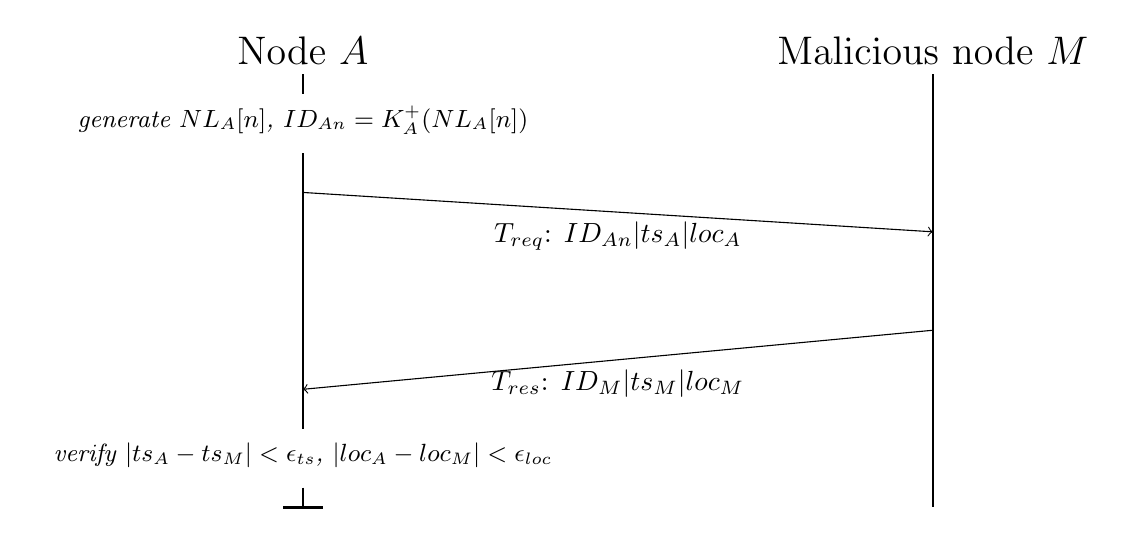
\begin{tikzpicture}
\coordinate (A_1) at (0,5.5);
\coordinate (A_2) at (0,5.25);
\coordinate (A_3) at (0,4.5);
\coordinate (A_8) at (0,1);
\coordinate (A_9) at (0,0.25);
\coordinate (A_12) at (0,0);
\coordinate (AF_L) at (-0.25,0);
\coordinate (AF_R) at (0.25,0);

\coordinate (B_1) at (8,5.5);
\coordinate (B_3) at (8,4.5);
\coordinate (B_8) at (8,3.25);
\coordinate (B_9) at (8,2.5);
\coordinate (B_12) at (8,0);

\draw[thick] (A_1)--(A_2) (A_3)--(A_8) (A_9)--(A_12) (AF_L)--(AF_R);
\draw[thick] (B_1)--(B_3) (B_3)--(B_9) (B_9)--(B_12);
\draw (A_1) node[above]{\Large Node $A$};
\draw (B_1) node[above]{\Large Malicious node $M$};

\draw (A_2) node[below,text centered]{\begin{tabular}{r}
\small{\textit{generate $NL_A[n]$, $ID_{An} = K^{+}_A(NL_A[n])$}}
\end{tabular}};

\coordinate (AX_1) at ($(A_3)-(0,0.5)$);
\coordinate (BX_1) at ($(B_3)-(0,1)$);
\draw[->] (AX_1) -- (BX_1) node[midway,below]
	{$T_{req}$: $ID_{An} | ts_A | loc_A$};

\coordinate (AX_2) at ($(A_3)-(0,3)$);
\coordinate (BX_2) at ($(B_8)-(0,1)$);
\draw[->] (BX_2) -- (AX_2) node[midway,below]
	{$T_{res}$: $ID_{M} | ts_M | loc_M$};
	
\draw (A_8) node[below,text centered]{\begin{tabular}{r}
\small{\textit{verify $|ts_A-ts_M| < \epsilon_{ts}$, $|loc_A-loc_M| < \epsilon_{loc}$}}
\end{tabular}};
\end{tikzpicture}}
\caption{An aborted transaction due to malicious node $M$}
\label{fig:aborted_transaction}
\end{figure}

\subsection{Verification}
\begin{minipage}{0.5\linewidth}
In the verification stage, a node tries to prove its location to a Verifier 3rd party, e.g. a bank. To do this, the node sends the Verifier a number of parameters, as shown in Figure \ref{fig:verify_request}:
\begin{itemize}[noitemsep,topsep=0pt]
	\item[] $\mathbf{ID_{An-1}}$ is the ID of $A$'s most recently published transaction.
	\item[] $\mathbf{KP_{An-1}}$ is $A$'s key packet from transaction $n-1$, and includes keys for as many transactions as $A$ feels is apropriate in order to receive verification.
	\item[] $\mathbf{loc}$ is $A$'s current claimed location for which it is seeking verification.
	\item[] $\mathbf{NP_{An-1}}$ is $A$'s \textit{Nonce Packet}, a list of the nonces used to generate $A$'s most recent IDs, from $n-1$.	
\end{itemize}
\end{minipage}
\hfill
\begin{minipage}[c]{0.5\linewidth}
\begin{figure}[H]
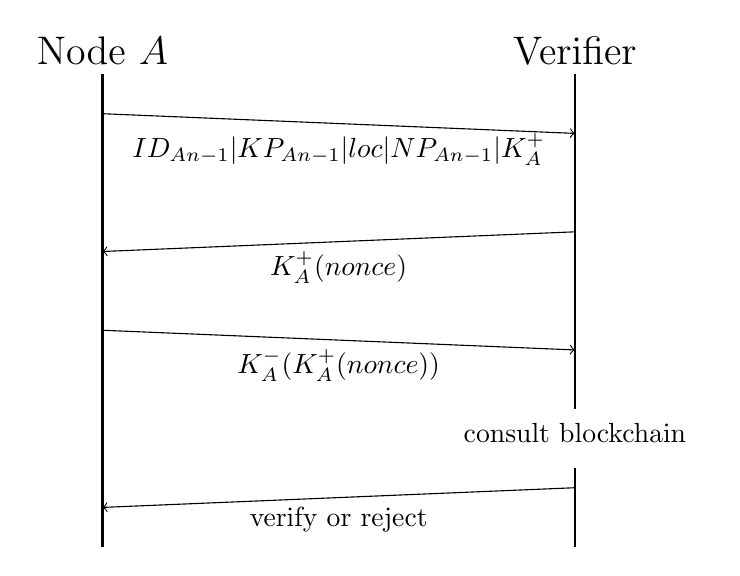
\begin{tikzpicture}
\coordinate (A_1) at (0,6);
\coordinate (A_2) at (0,0);

\coordinate (B_1) at (6,6);
\coordinate (B_2) at (6,1.75);
\coordinate (B_3) at (6,1);
\coordinate (B_4) at (6,0);

\draw[thick] (A_1)--(A_2);
\draw[thick] (B_1)--(B_2) (B_3)--(B_4);
\draw (A_1) node[above]{\Large Node $A$};
\draw (B_1) node[above]{\Large Verifier};

\coordinate (AX_1) at ($(A_1)-(0,0.5)$);
\coordinate (BX_1) at ($(B_1)-(0,0.75)$);
\draw[->] (AX_1) -- (BX_1) node[midway,below]
	{$ID_{An-1}|KP_{An-1}|loc|NP_{An-1}|K^{+}_A$};
	
\coordinate (AX_2) at ($(A_1)-(0,2.25)$);
\coordinate (BX_2) at ($(B_1)-(0,2)$);
\draw[->] (BX_2) -- (AX_2) node[midway,below]
	{$K^{+}_A(nonce)$};

\coordinate (AX_3) at ($(A_1)-(0,3.25)$);
\coordinate (BX_3) at ($(B_1)-(0,3.5)$);
\draw[->] (AX_3) -- (BX_3) node[midway,below]
	{$K^{-}_A(K^{+}_A(nonce))$};
	
\draw (B_2) node[below,text centered]{\begin{tabular}{r}
consult blockchain
\end{tabular}};

\coordinate (AX_2) at ($(A_1)-(0,5.5)$);
\coordinate (BX_2) at ($(B_1)-(0,5.25)$);
\draw[->] (BX_2) -- (AX_2) node[midway,below]
	{verify or reject};

\end{tikzpicture}
\caption{Verification request}
\label{fig:verify_request}
\end{figure}
\end{minipage}


The goal of the verification stage is for the Verifier to either accept or reject the location that the user is claiming. Given $ID_{An-1}$ and $KP_{An-1}$, a Verifier is able to retrieve $A$'s previous transactions, and the transactions of all of its alibi's.

The Verifier uses $NP_{An-1}$ and $K^{+}_A$ to prove that node $A$ was the author of all of the transactions he claims to be. This prevents a collusion attack whereby nodes could share common transactions between different proof chains. When walking chronologically backwards along $A$'s proof chain, the 3rd party will ensure that the ID used in transaction $m$ on the proof chain matches $K^{+}_A(NP_{An-1}[m])$.

There are a huge number of possible factors involved in reaching a conclusion from the data on the blockchain; some of these factors will likely be unique to certain verifiers, and kept secret to improve reliability and avoid gaming. Some simple example factors may include:
\begin{itemize}
	\item \textbf{Alibi credibility:} if each of the node’s alibi’s have little or no alibi’s themselves, then the node is likely attempting a poorly-constructed Sybil attack, and the verifier will reject his verification request.
	\item \textbf{Alibi reuse:} if the verifier can prove that alibi’s are being reused frequently, then it will reject the verification request.
	\begin{itemize}
		\item Due to transaction anonymity, the verifier may not always be able to tell if two alibi's are the same person or not. e.g. node $A$ could use node $B$ as an alibi, then wait for $B$ to complete $n$ more transactions, then use node $B$ again.
		\item This is not a viable attack on the verification system. Depending on the size of $n$, enough time may pass between both uses of node $B$ as an alibi that the transactions are no longer relevant.
	\end{itemize}
\end{itemize}

\subsection{Sybil attack}
This system is vulnerable to a Sybil attack, where a single physical node may create multiple \textit{pseudoidentities} \cite{sybil}. A suitably powerful node, or motivated attacker, could create enough pseudonyms to create a subnetwork of nodes, each creating malicious transactions with each other. This would allow an attacker to falsify a believable location proof.

It has been proven that a central certificate authority is the only method of preventing a Sybil attack \cite{sybil}. Other measures, such as web of trust, increase the difficulty involved in performing an attack, but the system remains vulnerable to a motivated attacker.

\newpage
\section{Evaluation}
In this paper, we have presented a model for a location proof system which aims to preserve privacy and prevent false proofs from being created.

\subsection{OTIT conformance}
We can compare our model to OTIT \cite{otit}, a list of features and requirements necessary for designing any secure location proof scheme. OTIT presents 8 such requirements:
\begin{enumerate}
\item[] \textbf{Chronological}: The chronological property of OTIT ensures that transactions are published in the order they were created. In our system we do not enforce this property at the time of transaction publication. This is to avoid revealing any transaction information to the miner nodes, therefore preserving the privacy of the transaction owner. Instead, we enforce this property at the time of verification. The chronological link created by adding $KL_{AT}(ID_{A-1}|ts_A)$ to the transaction will allow Verifier nodes to prove that the transaction is chronologically ordered, preserving OTIT's ``Chronological'' property.

\item[] \textbf{Order preserving}: This property states that the order of transactions cannot be modified after they are created. In our system, a blockchain is used to store transactions. In a blockchain, new blocks are added in a linear, chronological order, and cannot be modified so long as the majority of miners in the network are honest \cite{blueprint}. Therefore the transactions stored in these blocks satisfy the ``Order preserving'' property of OTIT. % in the dissertation i can discuss ordering within a block here (and go into detail about the merkle root etc)

\item[] \textbf{Verifiable}: This states that the proof, and the order or proofs, should be verifiable by a trusted auditor. In our case, a Verifier node is an auditor trusted by the mobile node seeking verification. A Verifier node may be operated by a bank, government, or any entity wishing to make use of our location proof system.

Our system inherently satisfies this property of OTIT, as Verifier nodes are required to verify or reject a mobile node's claimed location. This is done by examining the mobile node's chronological link of transactions, and recursing for each alibi used for each transaction along the chronological link until the Verifier can conclude if the transaction chain is valid or not.

\item[] \textbf{Tamper evident}: Our system is tamper evident. If a malicious node creates a successful transaction with an honest node, but modifies the transaction data before publishing, a Verifier node will reject the malicious transaction. This rejection will be on the grounds that the matching transaction, published by the honest node, contains contradictory data.

We assume the underlying security of the blockchain, so any malicious miner nodes will not be able to tamper with existing transaction data providing that the majority of CPU power in the mining system is owned by honest miners \cite{bitcoin}. Therefore the tamper evident property is satisfied.

\item[] \textbf{Privacy preserved}: This states that the user should have control over his level of privacy exposure when using the system. In our system, this is provided using \textit{Key Lists} \ref{sec:transactions}. We provide two keys for each transaction; $KL_{AT}[n]$ is used to encrypt the \textit{transaction data} for $A$'s $nth$ transaction, and $KL_{AL}[n]$ is used to encrypt the \textit{backwards chronological link} between $A$'s $nth$ transaction and transaction $n-1$.

To control his privacy, a user can choose only to reveal $KL_{AL}[n]$ for a specific transaction $n$. This may be useful if a user does not wish to reveal transaction data for transactions created within a certain distance of his house, for example. Hiding $KL_{AT}[n]$ while revealing $KL_{AL}[n]$ has the advantage of preserving the user's privacy while maintaining a clear backwards chronological link of transactions for the Verifier to follow, preserving both privacy and system consistency.

\item[] \textbf{Selective in-sequence privacy}: This is the requirement that any proof chain must support \textit{sub-set verification}, allowing a user to provide only a sub-set of proofs from his current proof chain for verification. Our system satisfies this property by using \textit{Key Packets} (section \ref{sssec:key_packets}).

In our system, a \textit{sub-set} of $A$'s proof chain can be defined as $KP_{An}$. The sub-set therefore begins with $ID_{An}$, and ends when there is no key $KL_{AL}[n-m]$ in $KP_{An}$ to decrypt the link to transaction $T_{An-m-1}$. 

\item[] \textbf{Privacy protected chronology}: This states that the proof system, which provides \textit{selective in-sequence privacy}, should also ensure that the user does not ``hide away'' important items within the subset. This is impossibnle in our system due to the use of backwards chronological linking between transactions, so our model satisfies this property.

\item[] \textbf{Convenience and derivability}: This requirement states that the verification process should be convenient, and the user should not burden the Verifier node with a huge load of data. In our system, the data is stored in a central blockchain that the Verifier has access to, and the user provides the Verifier only with decryption keys and indexes into a sub-section of this data. Therefore the data sent to from the user to the Verifier, $KP_{An}$, is quite small in size.

The Verifier has the freedom to decide how comprehensively to investigate the user's data; It can bound how deeply to investigate the graph of alibi's, if at all. We therefore satisfy this requirement by allowing the Verifier to choose how complex the verification process needs to be.
\end{enumerate}

\section{Conclusions}

\begin{thebibliography}{9}

\bibitem{brassil}
  J. Brassil, P.K. Manadhata,
  ``Verifying the Location of a Mobile Device User'',
  Proc. of MobiSec 2012,
  June 2012.

\bibitem{luo}
  Luo, W., Hengartner, U.,
  ``Proving your Location without giving up your Privacy'',
  Proceedings of the Eleventh Workshop on Mobile Computing Systems \& Applications,
  HotMobile 2010, Annapolis, Maryland, February 22 - 23, pp. 7–12. ACM,
  New York (2010)

\bibitem{khan}
  R. Khan, S. Zawoad, M. M. Haque, and R. Hasan,
  ```Who, When, and Where?' Location Proof Assertion for Mobile Devices'',
  Proceedings of the 28th Annual IFIP WG 11.3 Working Conference on Data and Applications Security and Privacy, ser. DBSec. IFIP,
  July 2014.
 
\bibitem{otit}
  Khan, R., Zawoad, S., Haque, M., Hasan, R.
  ``OTIT: Towards secure provenance modeling for location proofs'',
  Proc. of ASIACCS. ACM (2014)

\bibitem{sybil}
  Douceur, J.R.,
  ``The sybil attack'',
  Druschel, P., Kaashoek, M.F., Rowstron, A. (eds.) IPTPS 2002. LNCS, vol. 2429, pp. 251–260,
  Springer, Heidelberg (2002)

\bibitem{location-spoof}
  N. O. Tippenhauer, K. B. Rasmussen, C. Popper, and S. Capkun,
  ``iPhone and iPod location spoofing: Attacks on public WLAN-based positioning systems'',
  SysSec Technical Report,
  ETH Zurich, April, 2008

\bibitem{blueprint}
  M. Swan,
  ``Blockchain: Blueprint for a New Economy'',
  Sebastopol, CA,
  O’Reilly Media, 2015

\bibitem{bitcoin}
  S. Nakamoto,
  ``Bitcoin: A Peer-to-Peer Electronic Cash System'',
  2008

\end{thebibliography}

\end{document}